\documentclass[10pt,a4paper]{article}
\usepackage[a4paper, top=2cm, bottom=1.5cm, left=1.5cm, right=1.5cm]{geometry} % Задать размеры полей.
\usepackage[warn]{mathtext} % Русские символы в формулах. Нужно писать до пакета babel. Указывает, что в формулах используются символы кириллицы, которые по умолчанию печатаются прямым шрифтом.
\usepackage[T2A]{fontenc}
\usepackage[utf8]{inputenc}
\usepackage[russian]{babel}
\usepackage{amsmath}
\usepackage{amssymb}
\usepackage{graphicx}
\usepackage{floatrow}
\usepackage{booktabs}
\usepackage{wrapfig}
\usepackage{lipsum}
%\usepackage{subcaption}
\usepackage{fancyhdr}
\usepackage{multicol}
\usepackage{xcolor}

%multi-column
%\multicolumn{number cols}{align}{text} % align: l,c,r

%multi-row
\usepackage{multirow}

\newcommand{\figref}[1]{(См. рис. \ref{#1})}
\newcommand{\secref}[1]{(См. раздел. \ref{#1})}

\newcommand{\e}[1]{\text{$\cdot10^{#1}$}}
\newcommand{\m}{\; м}
\newcommand{\mm}{\; мм}
\newcommand{\um}{\; мкм}
\newcommand{\A}{\; А}
\newcommand{\uV}{\; мкВ}
\newcommand{\cels}{\; ^\circ С}

\pagestyle{fancy}
\fancyhead{}
\fancyhead[L]{\small Маслов А.С., Дедков Д.А., Экспериментальная проверка закона Стефана-Больцмана, и определение постоянных Стефана-Больцмана и Планка из анализа теплового излучения раскалённой вольфрамовой нити. МФТИ, 2023 г.}
\fancyhead[R]{}
\fancyfoot[C]{\thepage}

\renewcommand{\cot}{\text{ctg}}

\author{\normalsize Маслов Артём, Дедков Денис \\
	\normalsize группа Б01-108а \\
	\normalsize 04.09.2023}
\date{}

\usepackage{float}
\restylefloat{table}
\title{
	\Large Экспериментальная проверка закона Стефана-Больцмана, и определение постоянных Стефана-Больцмана и Планка из анализа теплового излучения раскалённой вольфрамовой нити \\ 
}

\addto\captionsrussian{\def\refname{Литература}}

\begin{document}
\maketitle
\begin{multicols}{2}
	
	\subsection*{Аннотация}
	В работе с помощью оптического термометра с исчезающей нитью измеряется температура раскалённой вольфрамовой нити при различной мощности, рассеиваемой в нити. Подтверждается линейная зависимость энергетической светимости от четвёртой степени температуры тела $T^4$. Определяются постоянные Стефана-Больцмана и Планка. Качественно исследуются излучения различных накалённых тел.
	
	\textbf{Ключевые слова:} закон Стефана-Больцмана, излучение АЧТ.
	
	\subsection*{Введение}
	
	\textit{Абсолютно чёрным телом (АЧТ)} называется тело, которое поглощает всё падающее на него излучение, но при этом само излучает энергию. 
	
	\textit{Потоком излучения} $\Phi$ называется мощность излучения, переносимая излучением через выбранную поверхность.
	$$
	\Phi = \frac{dE}{dt}
	$$
	где $E$ -- энергия, переносимая излучением.
	
	\textit{Плотностью потока излучения} $j(T)$ называется мощность излучения, переносимая излучением через единичную поверхность:
	$$
	j(T) = \frac{\Phi}{S}
	$$
	
	Согласно \textit{закону Стефана-Больцмана} интегральная плотность потока излучения связана с температурой тела формулой:
	\begin{equation}
		j(T) = \sigma T^4
		\label{eq:stefan_boltzman_law}
	\end{equation}
	где $\sigma$ -- постоянная Стефана-Больцмана. Согласно кватновой механике \cite[раздел~VIII]{labnik} постоянная Стефана-Больцмана связана с другими мировыми константами соотношением:
	\begin{equation}
		\sigma = \frac{2 \pi^5 k_Б^4}{15 c^2 h^3}
		\label{eq:const_stefan_boltzmann}
	\end{equation}
	
	Согласно квантовой механике АЧТ излучает неравномерно на разных частотах \cite[гл.~X]{Sivukhin4}. Для описания излучения на определённой частоте используется \textit{спектральная плотность потока излучения}:
	$$
	j_T(\omega) = \frac{d j(T)}{d \omega}
	$$
	Спектральная плотность потока излучения АЧТ вычисляется по \textit{формуле Планка}:
	$$
	j_T(\omega) = \frac{\hbar}{\left(2 \pi c \right)^2} \frac{\omega^3}{\exp \left(\frac{\hbar \omega}{k_Б T}\right) - 1}
	$$
	Из данной формулы можно получить зависимость спектральной плотности потока излучения от длины волны, если учесть, что $j_T(\omega) d\omega = j_T(\lambda) d\lambda$:
	$$
	j_T(\lambda) = \frac{\hbar c^2}{\lambda^5}  \frac{1}{\exp \left(\frac{h c}{\lambda k_Б T}\right) - 1}
	$$
	Типичный график зависимости спектральной плотности потока излучения $j_T(\lambda)$ АЧТ приведён на рисунке \ref{img:j_T(lambda)}:
	\begin{figure}[H]
		\centering
		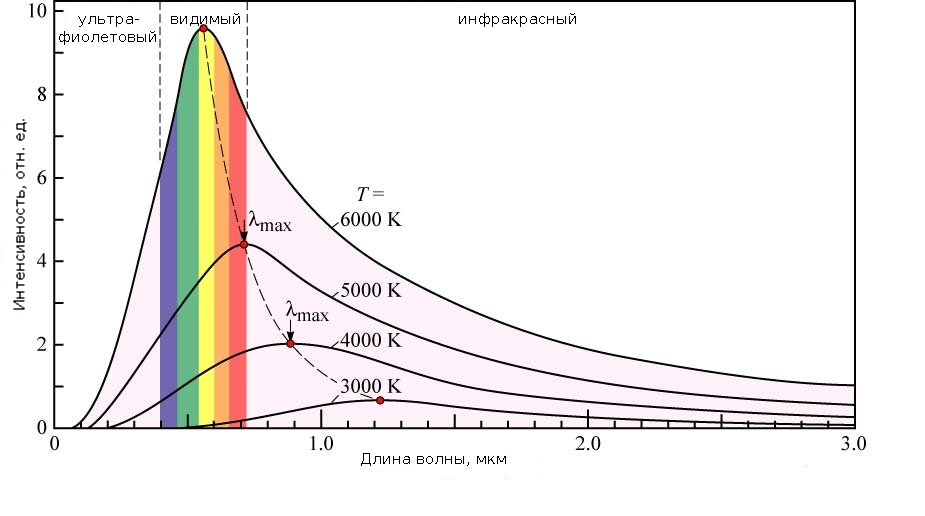
\includegraphics[width=1\textwidth]{images/j_t(lambda).jpg}
		\caption{График спектральной плотности потока излучения $j_T(\lambda)$ АЧТ для различных температур.}
		\label{img:j_T(lambda)}
	\end{figure}
	Спектральная плотность потока излучения имеет максимум $\lambda_{max}$. Формула, связывающая температуру тела и $\lambda_{max}$, называется \textit{законом смещения Вина}:
	$$
	T \lambda_{max} = 0,289776829 \dots \; К \cdot см
	$$
	
	\subsection*{Описание экспериментальной установки}
	
	Схема экспериментальной установки приведена на рисунке \ref{img:exp_scheme}:
	\begin{figure}[H]
		\centering
		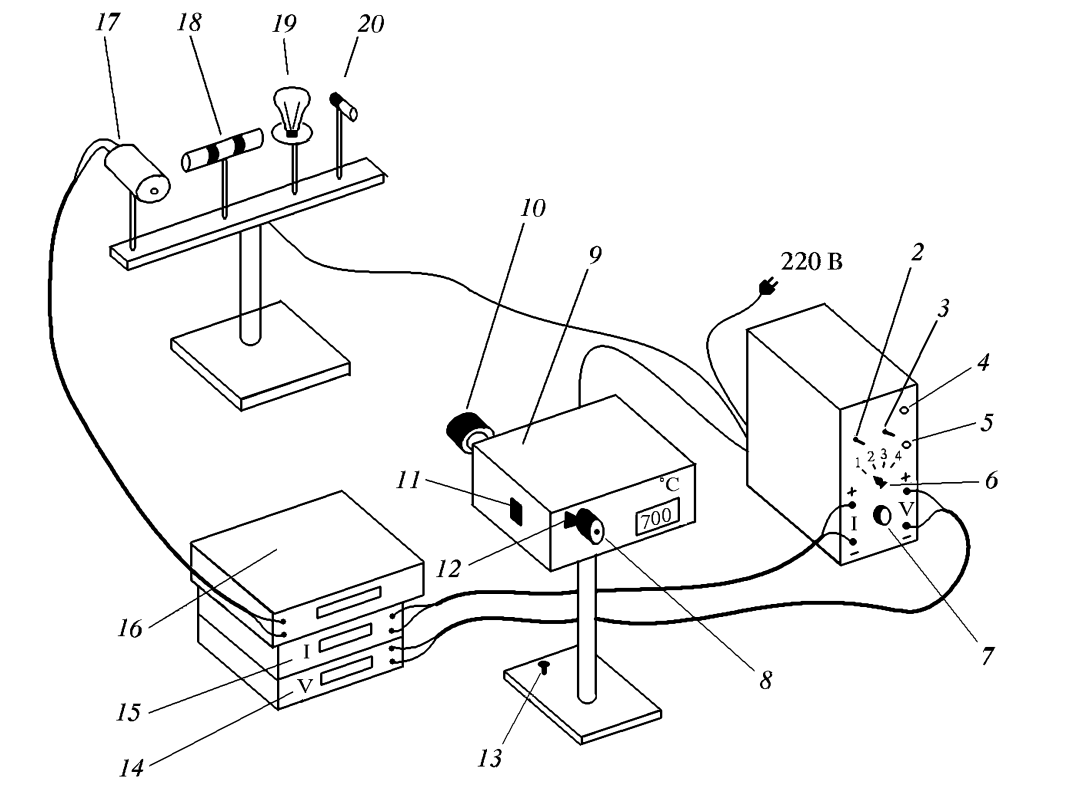
\includegraphics[width=1\textwidth]{images/exp_scheme.png}
		\caption{Схема экспериментальной установки.}
		\label{img:exp_scheme}
	\end{figure}
	
	С помощью оптического пирометра с исчезающей нитью 9 измеряется яркостная температура исследуемого тела. Объектив 10 используется для получения чёткого изображения предмета. С помощью окуляра 8 настраивается чёткое изображение исчезающей нити. Задвижка 11 позволяет вводить в оптическую систему пирометра серый светофильтр для изменения измеряемого диапазона температур. Без светофильтра измеряются температуры в диапазоне $700 \div 1200 \cels$, со светофильтром -- в диапазоне $1200 \div 2000 \cels$. С помощью переключателя 12 в оптическую систему можно вводить красный светофильтр.
	
	В работе исследуется излучение четырёх тел (17-20), закреплённых на специальном стенде. Модель АЧТ 17 представляет собой керамическую трубку длиной $50 \mm$, диаметром $3 \mm$, закрытую с одного конца. Трубка окружена теплоизоляционным кожухом. Стенки трубки нагреваются намотанной на неё нихромовой спиралью. Дно трубки излучает практически как абсолютно чёрное тело. Температура дна измеряется с помощью хромель-алюмелевой термопары, один конец которой вмонтирован в дно трубки, а другой находится при комнатной температуре. ЭДС термопары измеряется вольтметром 16. 18 -- керамическая трубка с закрепленными на ней кольцами из разных материалов с разной излучательной способностью. Трубка нагревается изнутри проводом до температуры примерно $1100 \cels$. Используется в работе для качественного сравнения испускательной способности различных материалов. 19 -- лампочка накаливания с вольфрамовой нитью. Используется для проверки закона Стефана-Больцмана и определения постоянных Планка и Стефана-Больцмана. 20 -- неоновая лампочка.
	
	Напряжение на исследуемые образцы подаётся с помощью блока питания, мощность регулируется ручкой 7, исследуемый образец можно выбирать с помощью переключателя 6. Напряжение на образце измеряется вольтметром 14, ток -- амперметром 15.
		
	\subsection*{Оборудование и приборы}
	\begin{enumerate}
		\item Оптический пирометр с исчезающей нитью Проминь М1. Диапазон измеряемых температур $800 \div 2000 \cels$, спектральный рабочий диапазон $0.655 \pm 0.01 \um$. Рабочее расстояние $0.7 \div \infty \m$.
		
		\item Хромель-алюминевая термопара. В диапазоне температур $900 \cels$ допустимое отклонение измеренной температуры от реальной составляет $\pm 7 \cels$, допустимое отклонение ЭДС $\pm 260 \uV$
		
		\item Набор исследуемых образцов, закреплённых на стенде. Подробное описание приведено в разделе <<Описание экспериментальной установки>>.
		
		\item Цифровые мультиметры GDM-8145. В режиме измерения постоянного напряжение погрешность измерения оценивается по формуле $\pm (0.03\% \cdot \text{<измеренное значение>} + 4 \text{ единицы младшего разряда})$. В режиме измерения постоянной силы тока на пределе $20 \A$ допустимое отклонение измеренных значений от реальных составляет $\pm (0.3\% \cdot \text{<измеренное значение>} + 2\text{ единицы младшего разряда})$.
		
		\item Лабораторный блок питания с возможность подключения различных образцов и регулируемой мощностью.
	\end{enumerate}
	
	\subsection*{Методика эксперимента}
	
	В начале работы проверяется, что пирометр правильно измеряет температуру. Для этого измеряется температура модели АЧТ с помощью термометра и термопары, показания приборов сверяются. ЭДС термопары $\varepsilon$ измеряется вольтметром и переводится в температуру $T_t$ согласно спецификации:
	$$
	T_t = \varepsilon / \psi + T_{л}
	$$
	где $\Psi = (39 \pm 1) \; мкВ/ ^\circ С$ -- постоянная термопары, $T_{л} = 22 \cels$ -- температура лаборатории.
	
	Для определение постоянной Стефана-Больцмана измеряется температура вольфрамовой нити и рассеиваемая в ней мощность. Предполагается, что в установившемся состоянии, вся подаваемая на вольфрамовую нить мощность $W$ рассеивается в виде излучения. Мощность $W$ определяется по закону Джоуля-Ленца и равна потоку излучения $\Phi$:
	$$
	\Phi = W = U \cdot I
	$$
	Пирометр измеряется \textit{яркостную температуру} нити. Под яркостной температурой понимается температура АЧТ, спектральная испускательная способность которого равна спектральной испускательной способности исследуемого тела на определённой длине волны. Для ограничения спектра излучения используется красный светофильтр пирометра. Для определения реальной температуры вольфрамовой нити по известной яркостной используется зависимость:
	
	\begin{figure}[H]
		\centering
		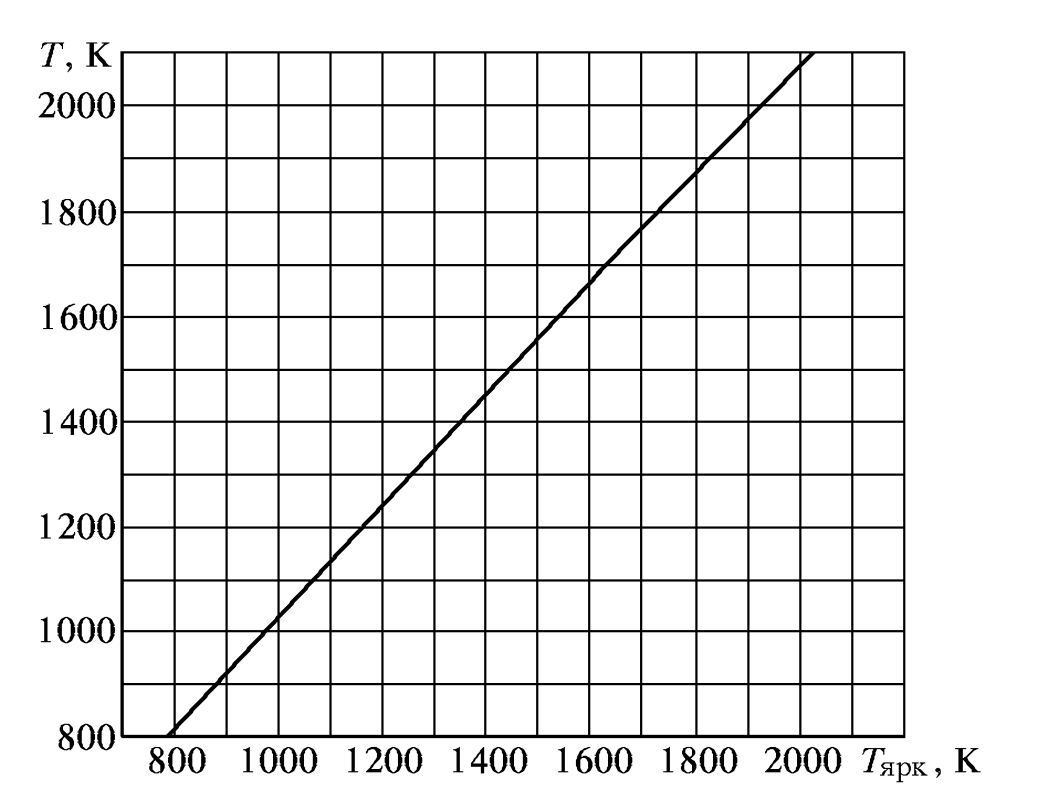
\includegraphics[width=0.8\textwidth]{images/wolfram_real_temp_brigh_temp.png}
		\caption{График зависимости реальной температуры вольфрама от яркостной.}
		\label{img:wolfram_real_temp_brigh_temp}
	\end{figure}
	
	Реальные тела не излучают как абсолютно чёрные. Если предположить, что спектральная излучательная способность исследуемого тела в $\varepsilon_T$ раз меньше спектральной излучательной способности АЧТ (\ref{eq:stefan_boltzman_law}), то излучаемая телом интегральная мощность будет вычисляться по формуле:
	\begin{equation}
		W = \varepsilon_T S \sigma T^4
		\label{eq:grey_stefan_boltzmann}
	\end{equation}
	где $S$ -- площадь излучающей поверхности тела, $\sigma$ -- постоянная Стефана-Больцмана. В данном соотношении учтено, что температура окружающей нить среды много меньше температуры нити. Тела, которые описываются такой моделью называются \textit{серыми}. Вольфрам лучше всего описывается моделью серого тела при высоких температурах $T > 1500 \cels$. 
	
	Для проверки закона Стефана-Больцмана предполагается степенная зависимость мощности излучения от температуры $W \propto T^n$ в законе (\ref{eq:grey_stefan_boltzmann}). По экспериментальным данным строится график зависимости мощности излучения от температуры в двойном логарифмическом масштабе, и находится коэффициент наклона прямой, равный показателю степени $n$:
	\begin{equation}
		\ln W = \ln (\varepsilon_T S \sigma) + n \ln T
		\label{eq:lin_grey_stefan_boltzmann}
	\end{equation}
	При определении показателя степени $n$ зависимостью $\varepsilon_T$ от температуры пренебрегаем. При определении постоянной Стефана-Больцмана зависимостью $\varepsilon_T(T)$ пренебречь нельзя, поэтому для каждого значения температуры вычисляется своя $\sigma$:
	\begin{equation}
		\sigma = \frac{W}{\varepsilon_T(T) \cdot S \cdot T^4}
		\label{eq:calc_const_stefan_boltzman}
	\end{equation}
	Преобразуя выражение (\ref{eq:const_stefan_boltzmann}) можно получить формулу для определения постоянной Планка:
	\begin{equation}
		h = \sqrt[3]{\frac{2 \pi^5 k_Б^4}{15 c^2 \sigma}}
		\label{eq:calc_const_planck}
	\end{equation}
	
	\subsection*{Обсуждение экспериментальных результатов}
		
	\subsubsection*{Проверка корректности работы оптического пирометра}
	
	В таблице \ref{table:term} приведены результаты измерений температуры АЧТ пирометром $T_p$ и термопарой $T_t$. $V$ -- ЭДС термопары.
	
	\begin{table}[H]
		\addtolength{\tabcolsep}{-4pt}
		\footnotesize
		\begin{tabular}{ccc}
\toprule
$T_{p}, ^oC$ & $V$, мВ & $T_{t}, ^oC$ \\
\midrule
947.0 & 36.4 & 936.5 \\
937.0 & 36.4 & 935.0 \\
939.0 & 36.3 & 934.5 \\
939.0 & 36.3 & 933.5 \\
938.0 & 36.3 & 933.5 \\
938.0 & 36.3 & 933.5 \\
938.0 & 36.3 & 933.3 \\
937.0 & 36.3 & 932.5 \\
939.0 & 36.3 & 932.5 \\
938.0 & 36.3 & 932.5 \\
\bottomrule
\end{tabular}
	
		\caption{Результаты измерений температуры АЧТ оптическим пирометром и термопарой.}
		\label{table:term}
	\end{table}
	
	Для определения случайной погрешности измерения температуры пирометром была проведена серия измерений. Эта погрешность учитывает влияние флуктуаций показаний пирометра и неточность человеческого глаза. Случайная ошибка измерения температуры $\sigma_{случ.} \sim 0.5 \cels$ мала по сравнению с инструментальной ошибкой пирометра $\sigma_{инстр.} \sim 10^\circ C$ в исследуемом диапазоне температур, и поэтому не будет учитываться в дальнейшем.
	
	Погрешность измерения термопары можно оценить как сумму случайной погрешности ($\sim0.015\;\text{мкВ}$) и ошибки приборной. Подсчет погрешности прибора для термопары класса K описан в ГОСТ-е: $\sigma_t = 0.0075t \sim 7\; ^oC$. Также определенную неточность в измерении финальной температуры вносит неизвестная температура комнаты $\sigma_{T_R} \sim 5\; ^oC$.
	
	$$\sigma_{T_t} \approx \sqrt{\sigma_{T_R}^2 + \sigma_t^2} \sim 9 ^oC.$$
	
	Относительная погрешность вычисленной температуры будет совпадать с относительной ошибкой измерения напряжения. 
	
	Итоговые значения температуры АЧТ, измеренные термопарой $T_t$ и пирометром $T_p$ соответственно:
	$$
	T_t = (934 \pm 9) \cels,\qquad T_p = (939 \pm 12) \cels.
	$$	
	Измеренные значения равны в пределах погрешности.
	
	\subsubsection*{Проверка закона Стефана-Больцмана}
	
	Результаты измерения яркостной температуры вольфрамовой нити $T$ при различной подаваемой на неё мощности $W$ приведены в таблице \ref{table:stefan_boltzmann}.
	
	\begin{table}[H]
		\addtolength{\tabcolsep}{-4pt}
		\footnotesize
		\begin{tabular}{cccc}
\toprule
$T, ^oC$ & $I$, А & $V$, В & $W$, Вт \\
\midrule
963.0 & 0.56 & 2.12 & 1.19 \\
1102.0 & 0.59 & 2.39 & 1.41 \\
1057.0 & 0.57 & 2.19 & 1.25 \\
1198.0 & 0.64 & 2.88 & 1.84 \\
1288.0 & 0.69 & 3.40 & 2.33 \\
1424.0 & 0.75 & 4.17 & 3.13 \\
1556.0 & 0.84 & 5.22 & 4.37 \\
1750.0 & 0.99 & 7.36 & 7.30 \\
1897.0 & 1.10 & 8.95 & 9.83 \\
\bottomrule
\end{tabular}

		\caption{Результаты измерения температуры вольфрамовой нити $T$ при различной подаваемой на неё мощности $W$.}
		\label{table:stefan_boltzmann}
	\end{table}
	
	Измеренная яркостная температура преобразуется в термодинамическую температуру с помощью графика зависимости, изображённого на рисунке \ref{img:wolfram_real_temp_brigh_temp}. По результатам измерений построим график зависимости потока излучения от температуры в обычном (рис. \ref{fig:wt}) и двойном логарифмическом масштабах (рис. \ref{fig:lnw_lnt}).
	
	\begin{figure}[H]
		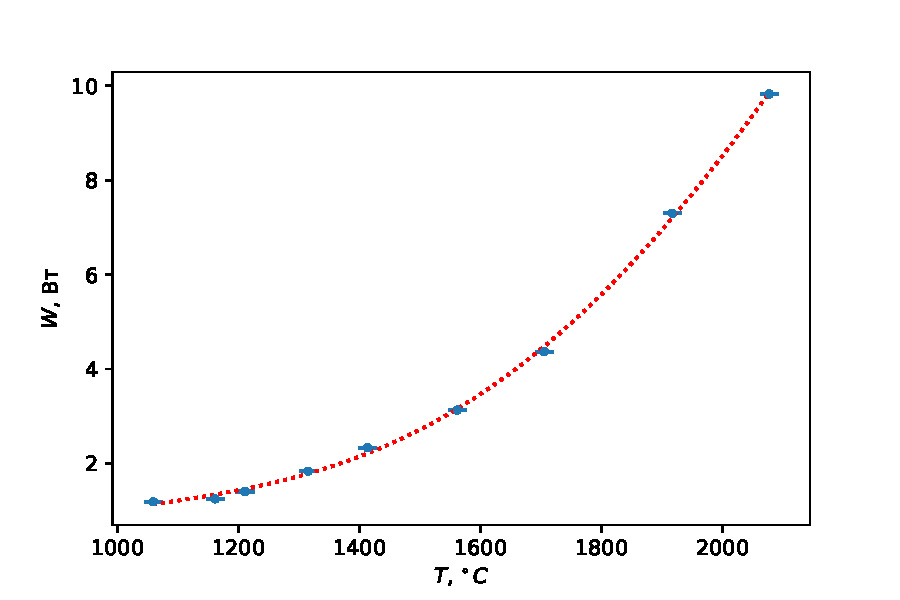
\includegraphics[width=1\textwidth]{gen/fig-wt.pdf}
		\caption{Зависимость потока излучения от температуры $W(T)$.}
		\label{fig:wt}
	\end{figure}

	\begin{figure}[H]
		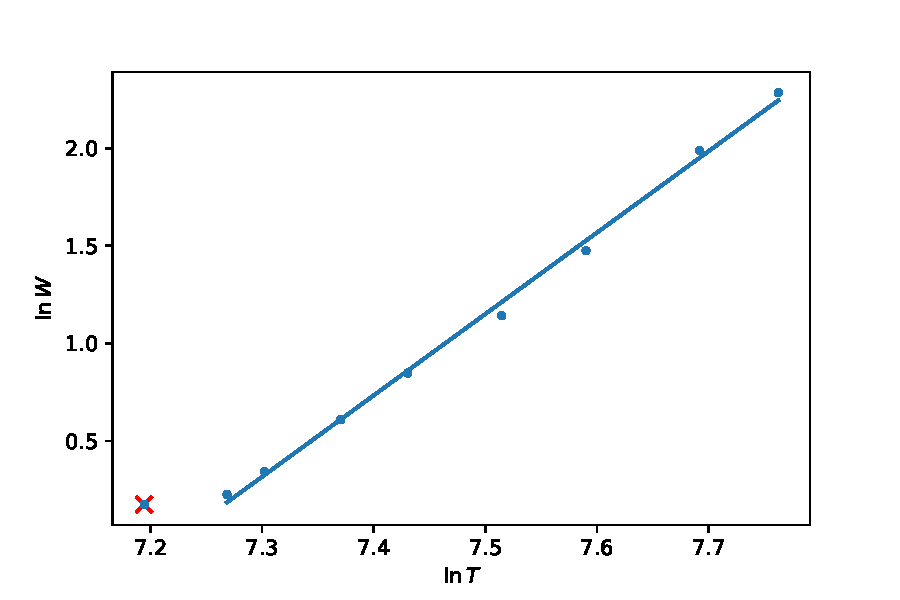
\includegraphics[width=1\textwidth]{gen/fig-linwt.pdf}
		\caption{Зависимость потока излучения от температуры $W(T)$ в двойном логарифмическом масштабе.}
		\label{fig:lnw_lnt}
	\end{figure}
	
	На графике в двойном логарифмическом масштабе аппроксимируем результаты измерений прямой $\ln W = b + n \ln T$ с помощью метода наименьших квадратов и определим показатель степени температуры $n$ в законе Стефана-Больцмана согласно формулы \ref{eq:lin_grey_stefan_boltzmann}. При аппроксимации прямой предполагается, что коэффициент серого тела $\varepsilon_T$ не зависит от температуры, поэтому первая точка отбрасывается, так как она плохо ложится на прямую. Коэффициенты МНК: \\
	$$n = 4.17 \pm 0.10,\;\; b = -30.2 \pm 0.7.$$
	
	\subsubsection*{Определение постоянной Стефана-Больцмана и Планка}
	
	На рисунке \ref{fig:epsilon_T} изображён график зависимости коэффициента серого тела вольфрама $\varepsilon_T$ от температуры $T$. Значения коэффициента $\varepsilon_T$ взяты из справочника \cite[стр.~236]{labnik}. Зависимость $\varepsilon_T$ аппроксимируется полиномом:
	
	$$ \varepsilon_T = -0.08 \cdot T^2 + 0.0002 \cdot T -1.6 \cdot 10^{-8}. $$
		
	\begin{figure}[H]
		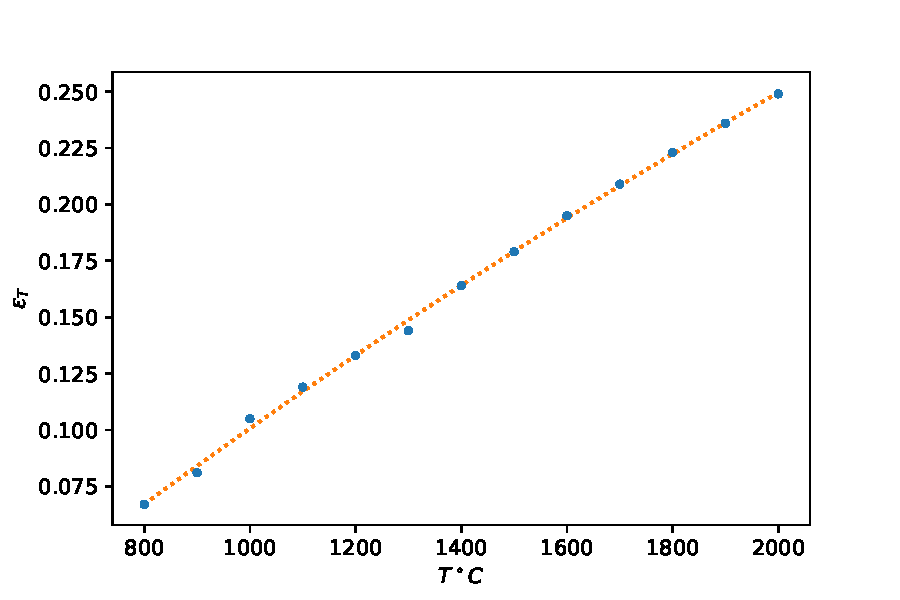
\includegraphics[width=1\textwidth]{gen/fig-epsilon.pdf}
		\caption{График зависимости коэффициента серого тела вольфрама $\varepsilon_T$ от температуры $T$.}
		\label{fig:epsilon_T}
	\end{figure}	 
	
	На рисунке \ref{fig:sigma} изображён график зависимости постоянной Стефана-Больцмана, вычисленной при различной температуре по формуле (\ref{eq:lin_grey_stefan_boltzmann}).
	
	
	\begin{figure}[H]
		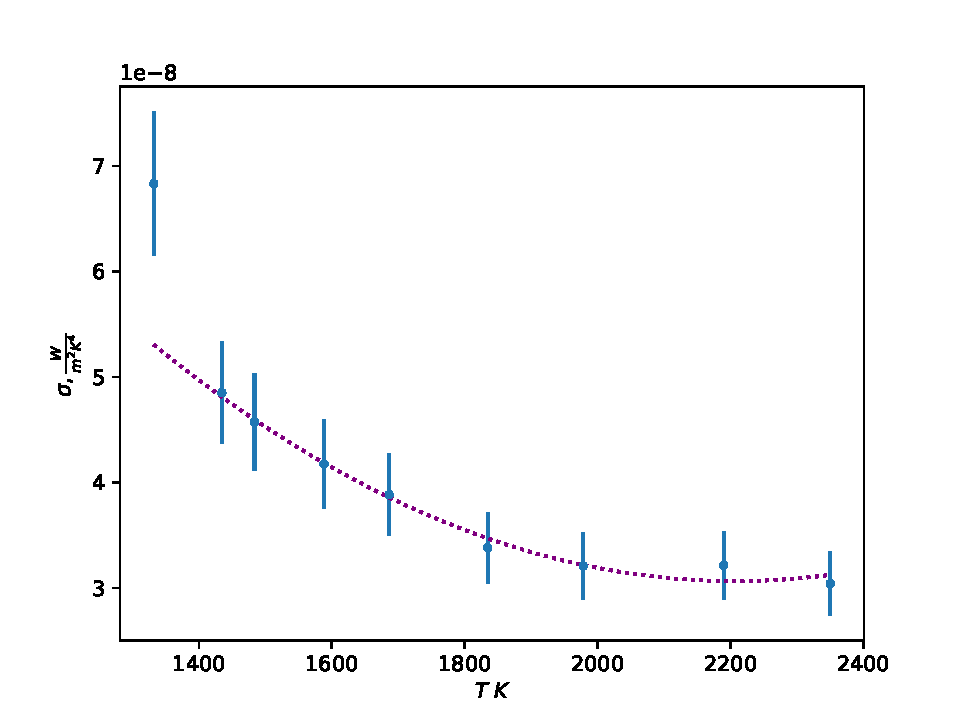
\includegraphics[width=1\textwidth]{gen/fig-sigma.pdf}
		\caption{График зависимости $\sigma(T)$.}
		\label{fig:sigma}
	\end{figure}	 
	
	Погрешность же, по правилам оценки погрешностей косвенных вычислений, можно оценить суммой относительных ошибок каждой величины:
	$$\varepsilon_\sigma \approx \sqrt{\varepsilon_S^2 + (4\varepsilon_T)^2} \sim 10 \%. $$\\

	Для вычисления постоянной Планка, определим постоянную Стефана-Больцмана, усреднив $\sigma_i$ для температур $T > 1800\; K$
	
	$$ \sigma = (3.2 \pm 0.3) \cdot 10^{-8} \frac{\text{Вт}}{\text{м}^2 \cdot K}.$$
	
	Погрешность постоянной Планка можно оценить по правилам нахождения погрешностей косвенных измерений:
	
	$$\varepsilon_h \approx \frac{1}{3} \varepsilon_\sigma.$$

	\subsection*{Выводы}
	
	В работе был экспериментально проверен закон Стефана-Больцмана. В пределах погрешности показатель степени температуры $n$ сходится с теоретическим значением:
	$$
	n = (3.92 \pm 0.18).
	$$
	
	Были определены постоянные Стефана-Больцмана $\sigma$ и Планка $h$. 
	$$
	\sigma = (3.2 \pm 0.3) \cdot 10^{-8} \frac{\text{Вт}}{\text{м}^2 \cdot K},$$ 
	$$h = (8 \pm 0.3) \cdot 10^{-34}\; \text{Дж} \cdot \text{с}.$$
	Измеренные постоянные по порядку сходятся с теоретическими значениями.
	
	\begin{thebibliography}{}
		\bibitem{labnik} \textbf{Ципенюк, Ю.М.} Лабораторный практикум по общей физике. Квантовая физика: Учеб. пособие для вузов./ Игошин~Ф.Ф., Самарский~Ю.А., Ципенюк~Ю.М.; Под. ред. Ципенюка~Ю.М. --- М.: Физматкнига, 2012. --- 464 с. ISBN 978-5-89155-206-7.
		\bibitem{Sivukhin4} \textbf{Сивухин, Д.В.} Общий курс физики: Учеб. пособие: Для вузов. В 5 т. Т.IV. Оптика. --- 4-е изд., стереот. --- М.: ФИЗМАТЛИТ, 2021. --- 792 с. ISBN 978-5-9221-1735-7 (Т. IV).
	\end{thebibliography}
\end{multicols}
\end{document}